%\documentclass[cprs.tex]{subfiles}
\setlength{\parskip}{1em}

\noindent In the following, the situation in which you are in this part is presented using an example. This example includes 3 rounds.

\noindent Please note: You will make your decisions not over 3, but over 5 rounds, and at the beginning of round 1 there will be 100 trees in the forest.

\section*{Round 1}
\subsection*{State of the forest at the beginning of round 1}
At the beginning of the round, there are 65 trees in the forest.
\begin{center}
   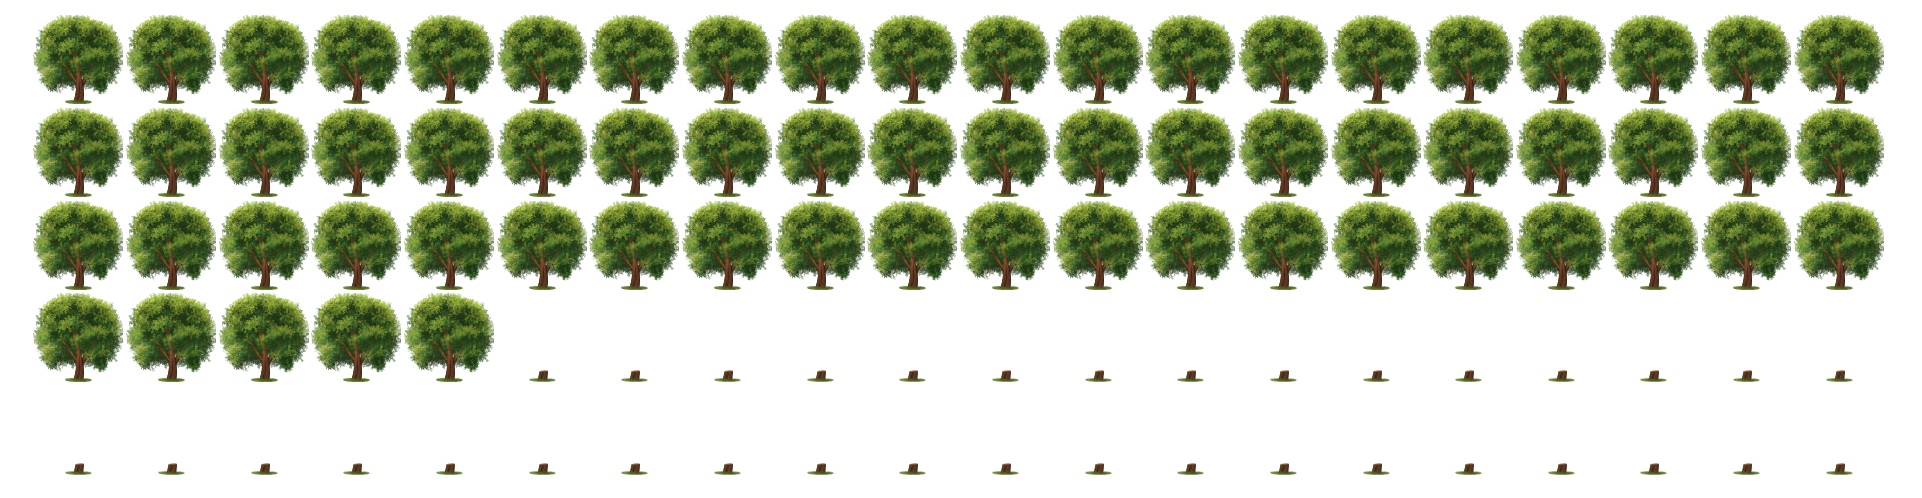
\includegraphics[width=16cm]{../bld/graphs/A. Round1a.png}
\end{center}

\subsection*{Decisions of the three group members}

\noindent Group member \textbf{A} takes 5 trees.

\noindent Group member \textbf{B} takes 2 trees.

\noindent Group member \textbf{C} takes 3 trees.

\noindent The entire group has taken 10 trees.

\noindent \textbf{Please note: Later, you will only have the information about how many trees you and your group have taken as a whole.}

\subsection*{State of the forest after removal}

At the beginning of the round, there are 65 trees in the forest. The group takes 10 trees. After the removal, 55 trees are available.
\begin{center}
   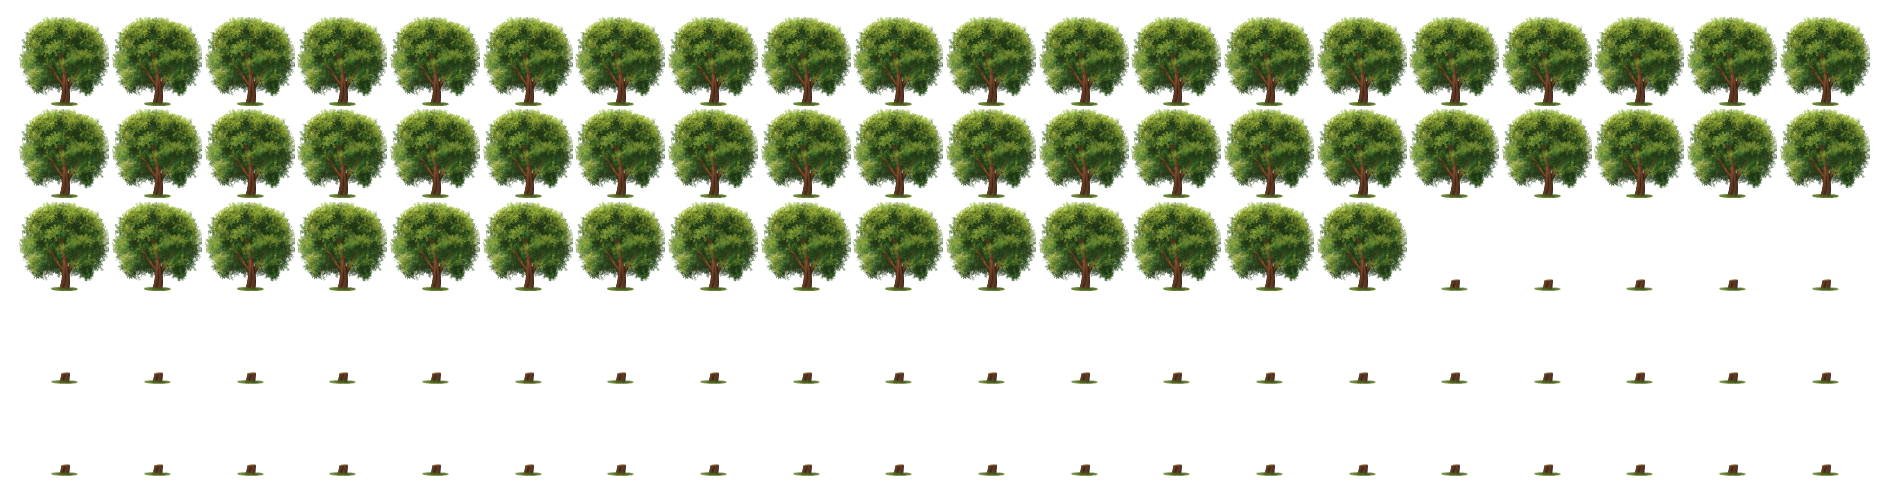
\includegraphics[width=16cm]{../bld/graphs/A. Round1b.png}
\end{center}

\subsection*{Earnings in round 1}

\textbf{Group member A}

\noindent As a starting credit, group member A receives 50 points.

\noindent Group member A receives 10 points for the trees taken. In this round, group member A receives a total of 10 points.

\noindent After this round, group member A has 50 points starting credit + 10 points from trees taken = 60 points.

\noindent \textbf{Group member B}

\noindent As a starting credit, group member B receives 50 points.

\noindent Group member B receives 4 points for the trees taken. In this round, group member B receives a total of 4 points.

\noindent After this round, group member B has 50 points starting credit + 4 points from removed trees = 54 points.

\noindent\textbf{Group member C}

\noindent As a starting credit, group member C receives 50 points.

\noindent Group member C receives 6 points for the removed trees. In this round, group member C receives a total of 6 points.

\noindent After this round, group member C has 50 points starting credit + 6 points from removed trees = 56 points.

\subsection*{State of the forest at the end of round 1}

After the removal, 55 trees are available. Due to the growth rate of 10\%, 5.5 trees grow back. There are 60.5 trees at the end of the round.

\begin{center}
   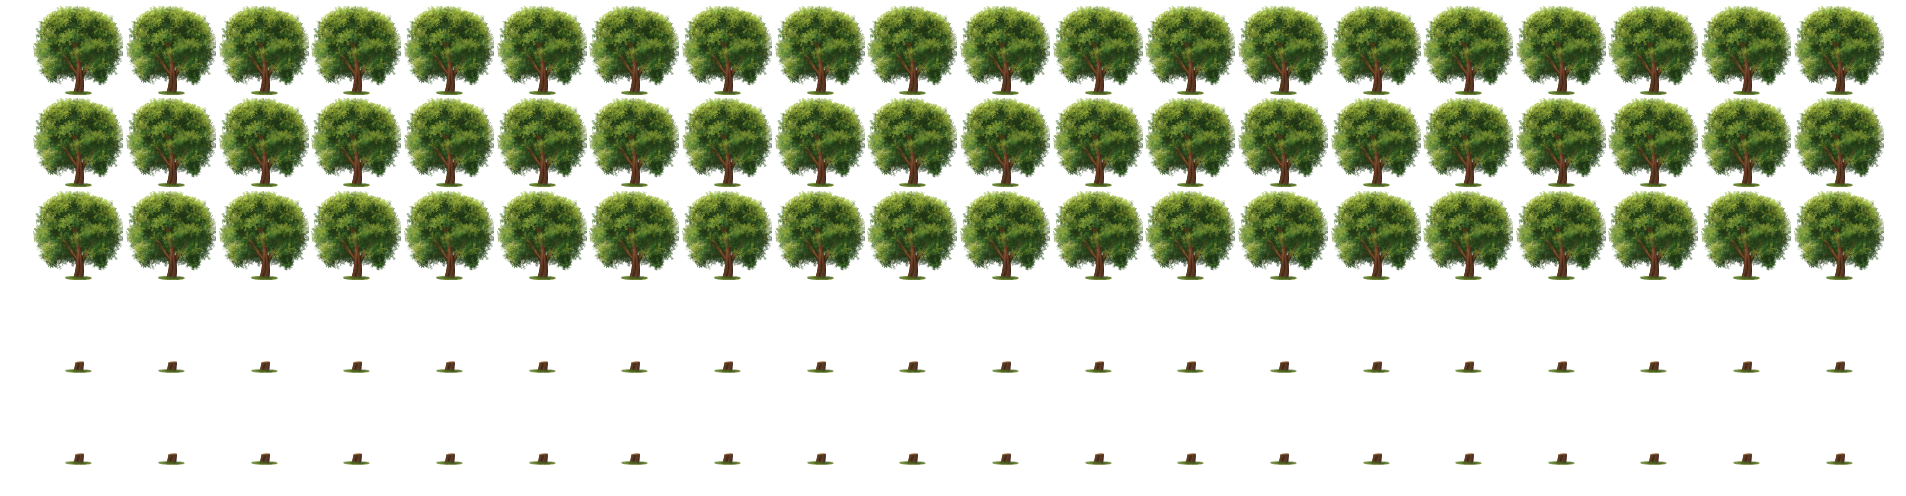
\includegraphics[width=16cm]{../bld/graphs/A. Round1c.png}
\end{center}

\section*{Round 2}

At the beginning of the round, there are 60.5 trees in the forest.
\begin{center}
   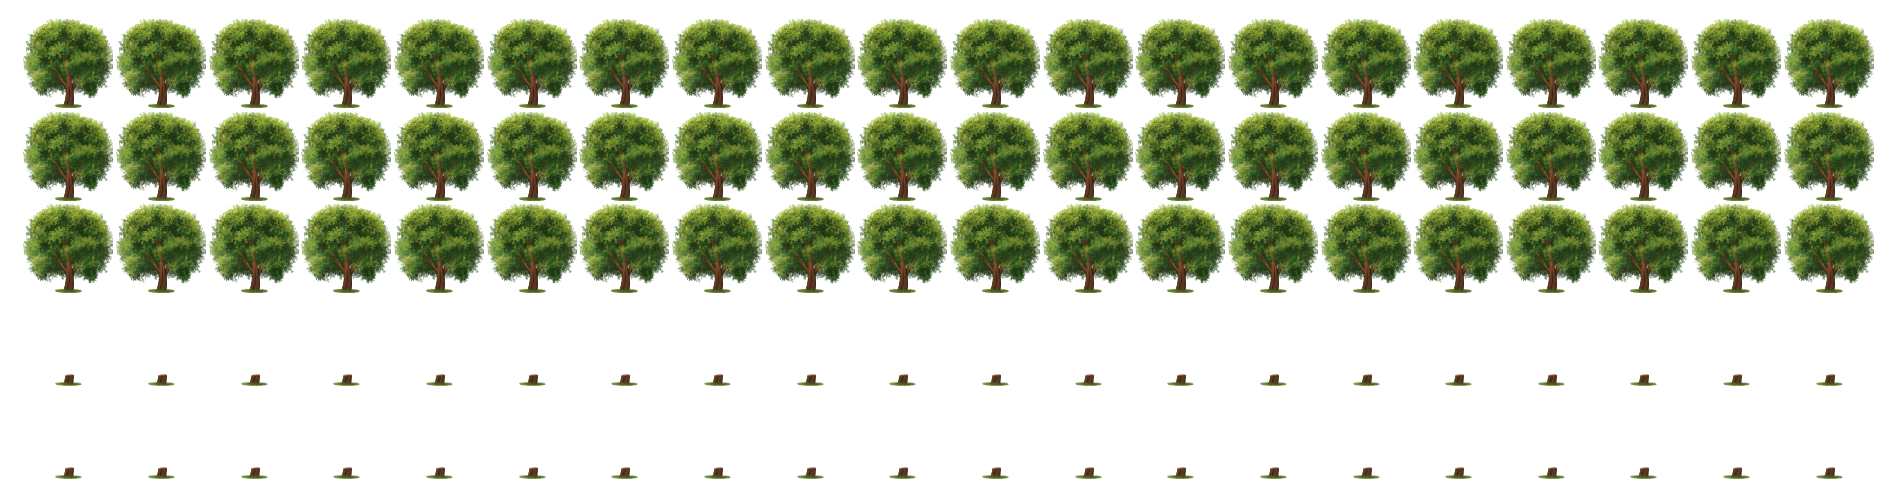
\includegraphics[width=16cm]{../bld/graphs/A. Round2a.png}
\end{center}

\noindent \textbf{Please note: Even if the specified number of current trees at the beginning of the round e.g. 60.5 trees, only 60 fully grown trees are displayed in the graph. You can only remove fully grown trees.}

\noindent Decisions of the three group members

\noindent Group member \textbf{A} takes 0 trees.

\noindent Group member \textbf{B} takes 0 trees.

\noindent Group member \textbf{C} takes 0 trees.

\noindent The entire group has thus removed 0 trees.


\subsection*{State of the forest after removal}

At the beginning of the round, there are 60.5 trees in the forest. The group takes 0 trees. After the removal, there are 60.5 trees.
\begin{center}
   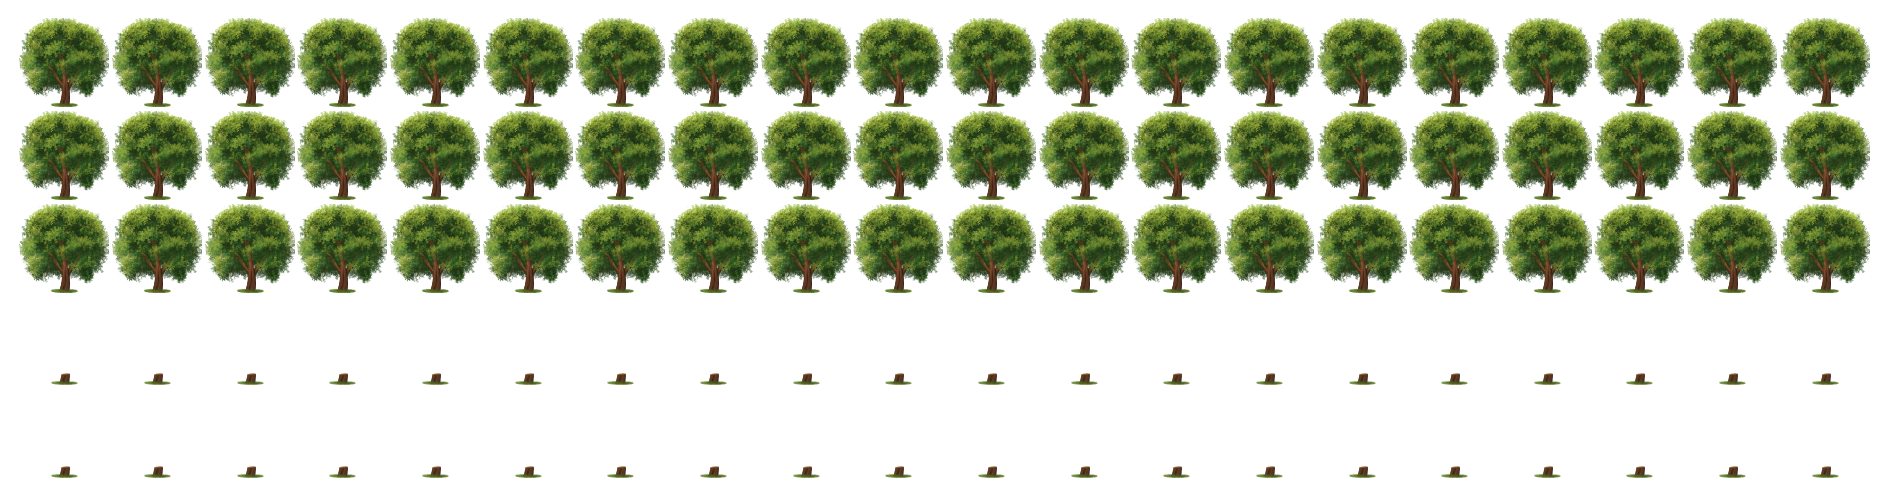
\includegraphics[width=16cm]{../bld/graphs/A. Round2b.png}
\end{center}

\subsection*{Earnings in round 2}

\noindent\textbf{Group member A}

\noindent From the previous round, group member A has 60 points.

\noindent Group member A receives 0 points for the trees taken. In this round, group member A receives a total of 0 points.

\noindent After this round, group member A has 60 points from the previous round + 0 points from removed trees = 60 points.

\noindent \textbf{Group member B}

\noindent From the previous round, group member B has 54 points.

\noindent Group member B receives 0 points for the trees removed. In this round, group member B receives a total of 0 points.

\noindent After this round, group member B has 54 points from the previous round + 0 points from removed trees = 54 points.

\noindent \textbf{Group member C}

\noindent From the previous round, group member C has 56 points.

\noindent Group member C receives 0 points for the removed trees. In this round, group member C receives a total of 0 points.

\noindent After this round, group member C has 56 points from the previous round + 0 points from removed trees = 56 points.

\subsection*{State of the forest at the end of round 2}

\noindent After the removal, there are 60.5 trees. Due to the growth rate of 10\%, 6.05 trees grow back. At the end of the round there are 66.55 trees.
\begin{center}
   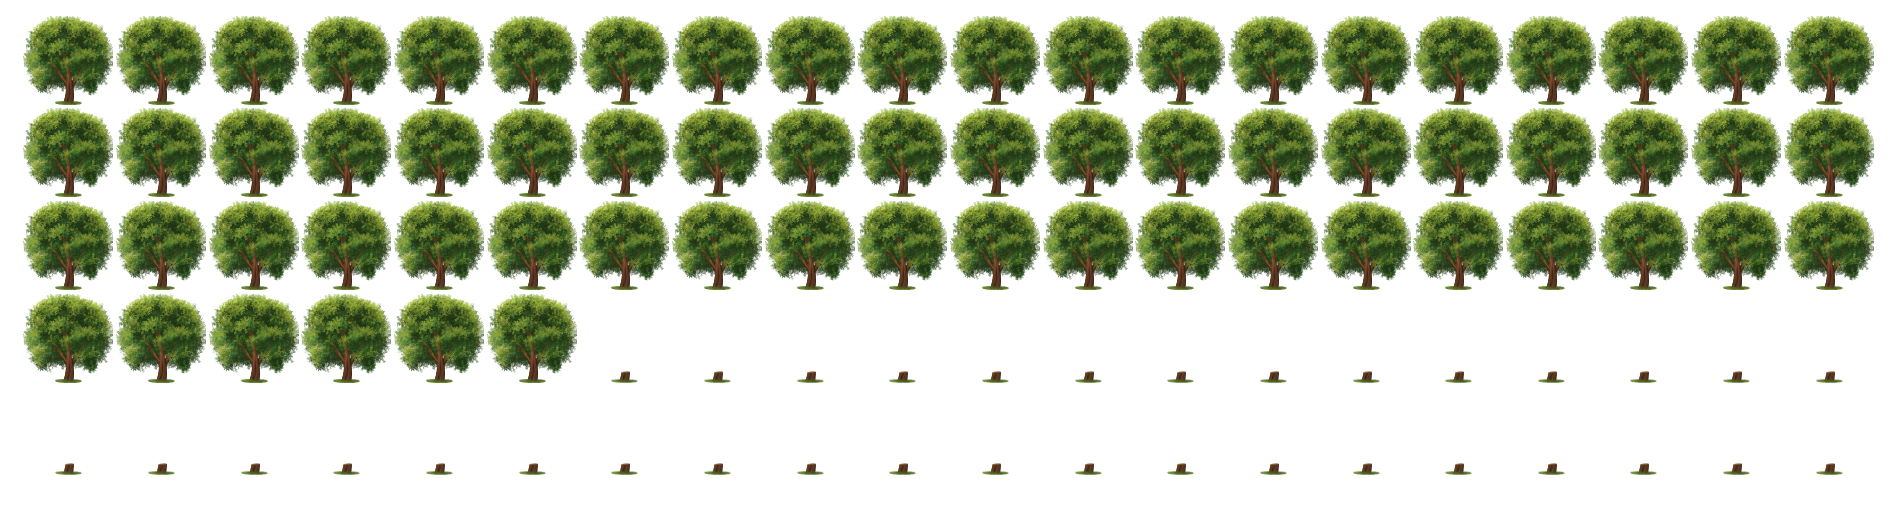
\includegraphics[width=16cm]{../bld/graphs/A. Round2c.png}
\end{center}

\section*{Round 3}

\noindent At the beginning of the round, there are 66.55 trees in the forest.
\begin{center}
   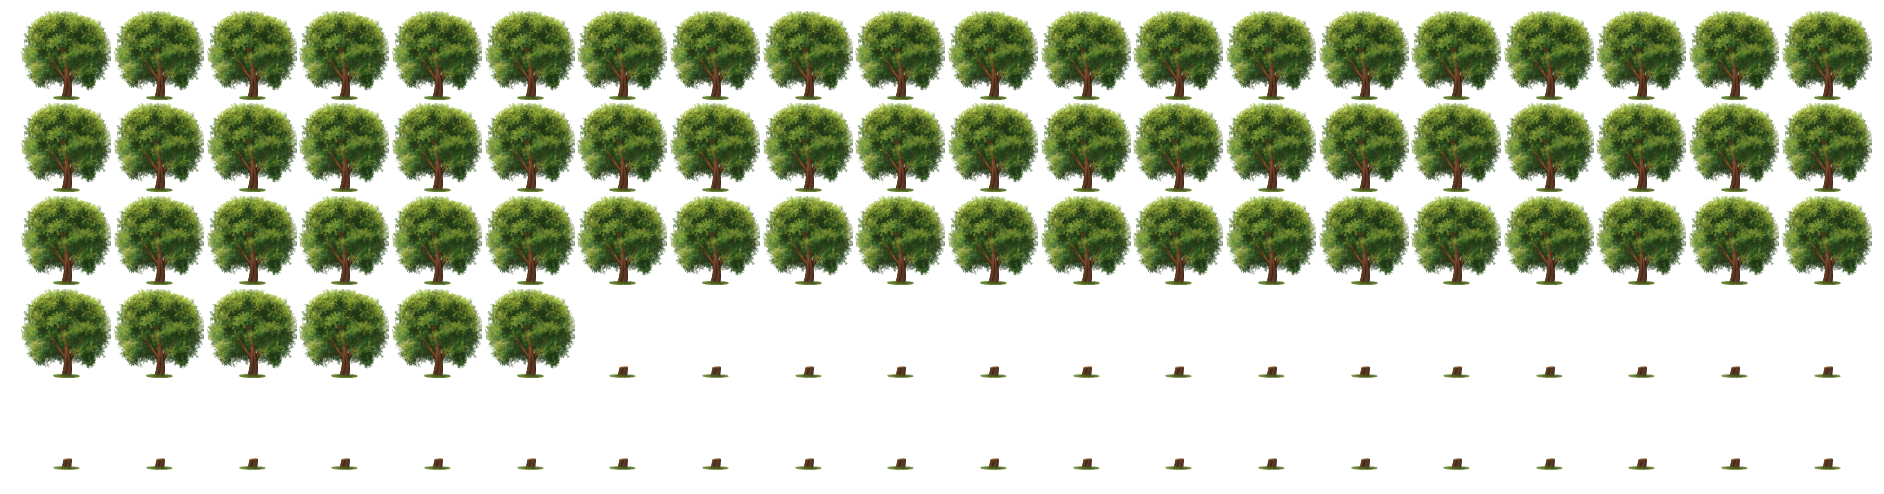
\includegraphics[width=16cm]{../bld/graphs/A. Round3a.png}
\end{center}

\subsection*{Decisions of the three group members}

\noindent Group member \textbf{A} takes 1 tree.

\noindent Group member \textbf{B} takes 3 trees.

\noindent Group member \textbf{C} takes 7 trees.

\noindent The entire group has taken 11 trees.

\subsection*{State of the forest after removal}

\noindent At the beginning of the round, there are 66.55 trees in the forest. The group takes 11 trees. After the removal, 55.55 trees are available.
\begin{center}
   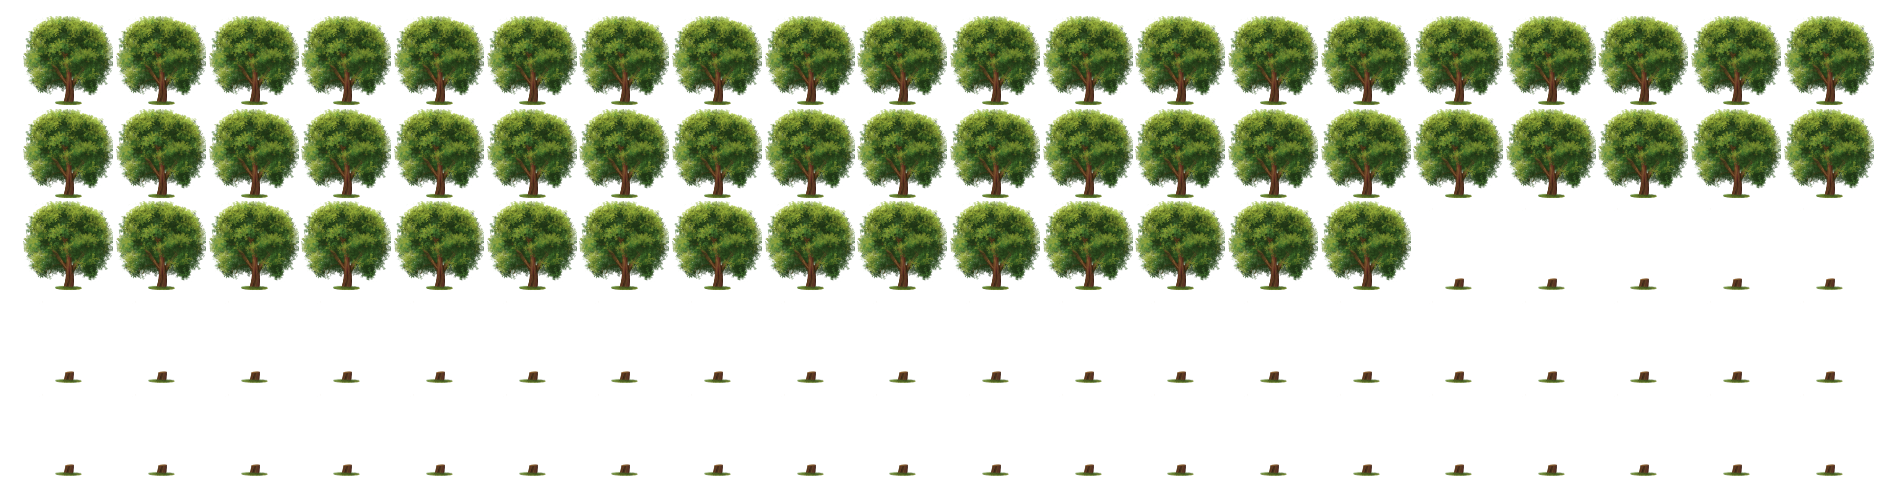
\includegraphics[width=16cm]{../bld/graphs/A. Round3b.png}
\end{center}

\subsection*{Earnings in round 3}

\noindent \textbf{Group member A}

\noindent From the previous round, group member A has 60 points.

\noindent Group member A receives 2 points for the trees taken. In this round, group member A receives a total of 2 points.

\noindent After this round, group member A has 60 points from the previous round + 2 points from removed trees = 62 points.

\noindent \textbf{Group member B}

\noindent From the previous round, group member B has 54 points.

\noindent Group member B receives 6 points for the trees taken. In this round, group member B receives a total of 6 points.

\noindent After this round, group member B has 54 points from the previous round + 6 points from removed trees = 60 points.

\noindent \textbf{Group member C}

\noindent From the previous round, group member C has 56 points.

\noindent Group member C receives 14 points for the trees taken. In this round, group member C receives a total of 14 points.

\noindent After this round, group member C has 56 points from the previous round + 14 points from removed trees = 70 points.

\subsection*{State of the forest at the end of round 3}

\noindent After the removal, 55.55 trees are available. Due to the growth rate of 10\%, 5.56 trees grow back. At the end of the round there are 61.11 trees.
\begin{center}
   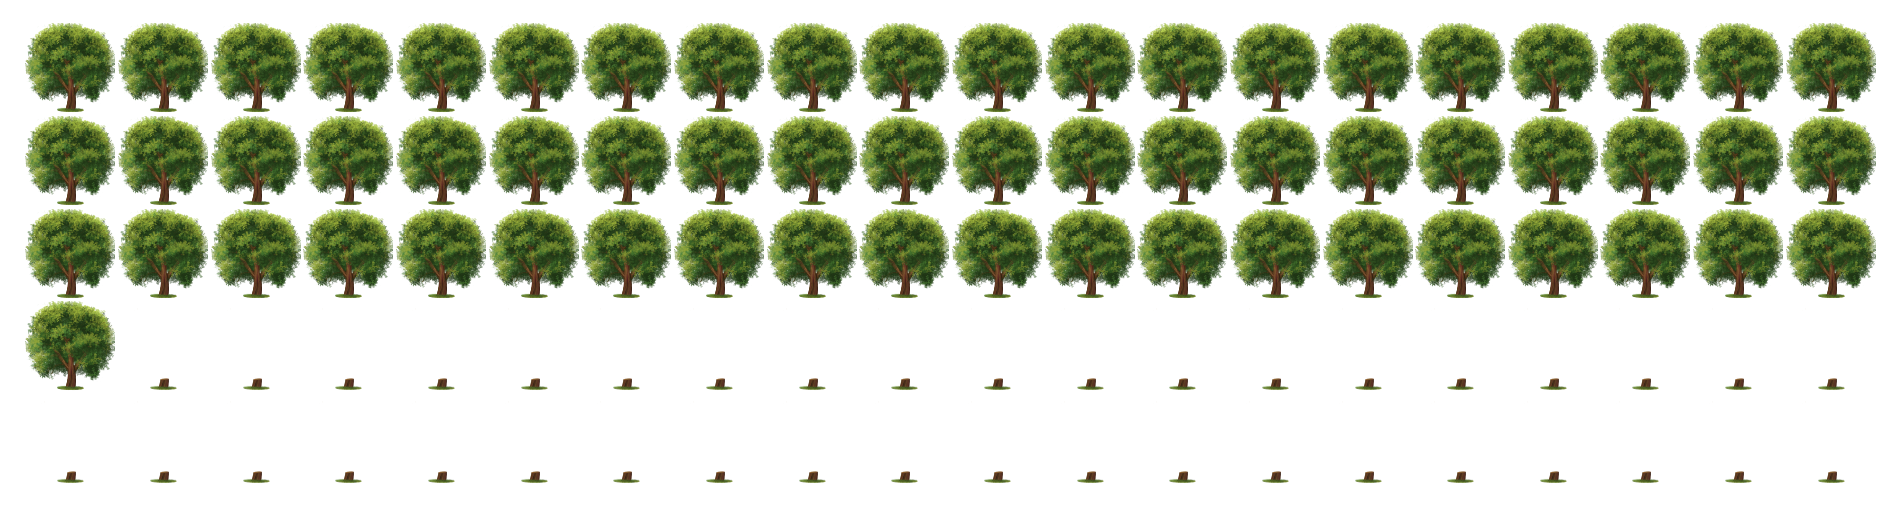
\includegraphics[width=16cm]{../bld/graphs/A. Round3c.png}
\end{center}

\subsection*{Total payout after round 3}

\noindent Assume that round 3 is the last round. Now each group member receives an equal share of the value of the forest. 61.11 trees have remained in the forest. These have a value of 122.22 points. Now the value is doubled to 244.44 points.

\noindent Each group member now receives an equal share of 244.44/3 = 81.48 points.

\noindent \textbf{Group member A }receives a total of 50 points (starting credit) + 10 points (round 1) + 0 points (round 2) + 2 points (round 3) + 81.48 points (share of the value of the forest at the end of the last round) = 143.48 points.

\noindent \textbf{Group member B} receives a total of 50 points (starting credit) + 4 points (round 1) + 0 points (round 2) + 6 points (round 3) + 81.48 points (share of the value of the forest at the end of the last round) = 141.48 points.

\noindent \textbf{Group member C} receives a total of 50 points (starting credit) + 6 points (round 1) + 0 points (round 2) + 14 points (round 3) + 81.48 points (share of the value of the forest at the end of the last round) = 151.48 points.
